%%%%%%%%%%%%%%%%%%%%%%%%%%%%%%%%%%%%%%%%%
%This poster template was modified by Samanthule Nola for use in the University of Michigan 2015 Engineering Graduate Symposium.
%August 7, 2015
%\a0poster Portrait Poster
% LaTeX Template
% Version 1.0 (22/06/13)
%
% The a0poster class was created by:
% Gerlinde Kettl and Matthias Weiser (tex@kettl.de)
%
% This template has been downloaded from:
% http://www.LaTeXTemplates.com
%
% License:
% CC BY-NC-SA 3.0 (http://creativecommons.org/licenses/by-nc-sa/3.0/)
%
%%%%%%%%%%%%%%%%%%%%%%%%%%%%%%%%%%%%%%%%%

%----------------------------------------------------------------------------------------
%	PACKAGES AND OTHER DOCUMENT CONFIGURATIONS
%----------------------------------------------------------------------------------------

\documentclass[landscape,a0a,final]{a0poster}
%a0 size is 841 X 1189  = 33.11 X 46.811 in., but we want a 30 X 40 in poster,so need to scale down the poster size

\usepackage{multicol} % This is so we can have multiple columns of text side-by-side
\usepackage{multirow}
\columnsep=100pt % This is the amount of white space between the columns in the poster
\columnseprule=0pt % This is the thickness of the black line between the columns in the poster

\usepackage[svgnames]{xcolor} % Specify colors by their 'svgnames', for a full list of all colors available see here: http://www.latextemplates.com/svgnames-colors
%\usepackage{xcolor}

%\usepackage{times} % Use the times font
\usepackage{helvet} % Use a font similar to Arial if using LaTeX or if running on a machine without commercial fonts available
\renewcommand{\familydefault}{\sfdefault}
% if using XeLaTex on mac or windows, the following lines should give true Ariel font
%\usepackage{fontspec}
%\setmainfont{Arial}

\usepackage{graphicx} % Required for including images
\usepackage{epstopdf}
\graphicspath{{./figures/}} % Location of the graphics files
\usepackage{booktabs} % Top and bottom rules for table
\usepackage[font=small,labelfont=bf]{caption} % Required for specifying captions to tables and figures
\usepackage{amsfonts, amsmath, amsthm, amssymb, amsthm} % For math fonts, symbols and environments
%\usepackage[ruled]{algorithm2e}
\usepackage{wrapfig} % Allows wrapping text around tables and figures
%\usepackage{algorithm2e}
\usepackage{fancybox}
\usepackage{bibentry}

\usepackage[usenames,dvipsnames]{pstricks}
\usepackage{epsfig}
\usepackage{pst-grad} % For gradients
\usepackage{pst-plot} % For axes
\usepackage[space]{grffile} % For spaces in paths
\usepackage{etoolbox}
\usepackage{lipsum}
\makeatletter % For spaces in paths
\patchcmd\Gread@eps{\@inputcheck#1 }{\@inputcheck"#1"\relax}{}{}
\makeatother

% Modifications to add a colored block behind section headings
%\definecolor{maiz}{cmyk}{1.18,14.9,99.61,0}%make maiz color
\definecolor{maiz}{cmyk}{0,100,100,20}%make maiz color
%\definecolor{mblue}{cmyk}{100,91.37,30.98,25.49}%make maiz color
\definecolor{mblue}{cmyk}{0,100,100,20}%make maiz color
%\definecolor{nmaiz}{HTML}{FFCB05}
\definecolor{nmaiz}{HTML}{AC0303}
%\definecolor{nblue}{HTML}{00274C}
\definecolor{nblue}{HTML}{9B0F0F}
\usepackage[explicit]{titlesec}
\titleformat{\section}
{\fontsize{40}{45}\selectfont}{}{0em}{\colorbox{mblue}{\parbox{\dimexpr\textwidth-2\fboxsep\relax}{\textcolor{maiz}{\thesection\quad#1}}}}
\titleformat{name=\section,numberless}
{\fontsize{40}{45}\selectfont\bfseries}{}{0em}{\colorbox{nblue}{\parbox[c][2cm]{\dimexpr\linewidth-2\fboxsep\relax}{\textcolor{white}{#1}}}}

\usepackage{array}
\newcommand{\PreserveBackslash}[1]{\let\temp=\\#1\let\\=\temp}
\newcolumntype{C}[1]{>{\PreserveBackslash\centering}p{#1}}
\newcolumntype{R}[1]{>{\PreserveBackslash\raggedleft}p{#1}}
\newcolumntype{L}[1]{>{\PreserveBackslash\raggedright}p{#1}}

%%%%%%%%%%%%%%%%%%%%%%%%%%%%%%%%%%
%IMPORTANT NOTE ABOUT PAGE SIZE:
%The used area is 28 X 38 inches, please do not put content in the margins, and please crop the extra white space from the rendered pdf leaving 1 inch margins on all sides for a 30X40 inch poster.

%\special{papersize=30in,40in} %these commanmds don't work in a0poster template
%\setlength{\paperwidth}{30in}
%\setlength{\paperheight}{50in}
\setlength{\paperwidth}{46in}
\setlength{\paperheight}{36in}
\setlength{\textwidth}{44in}
\setlength{\textheight}{34in}
\setlength\parindent{0pt}

\usepackage[plain]{algorithm}
\usepackage{algorithmic}
\renewcommand{\algorithmicensure}{\textbf{Output:}}

% LaTeX packages
\usepackage{algorithm}
\usepackage{algorithmic}
\usepackage{amsmath}
\usepackage{amssymb}
\usepackage{amsthm}
\usepackage[english]{babel}
\usepackage[singlelinecheck=false]{caption}
\usepackage[colorlinks=true,citecolor=blue,linkcolor=blue]{hyperref}
\usepackage{natbib}
\usepackage{thmtools}
\usepackage{tikz}
\usepackage{color}
\usepackage{comment}
\usepackage{commath}
\usepackage{dsfont}
\usepackage[accepted]{icml2019}  % Remove [accepted] for ICML submission (to make the paper anonymous).

% TikZ packages
\usetikzlibrary{arrows}
\usetikzlibrary{angles}
\usetikzlibrary{backgrounds}
\usetikzlibrary{calc}
\usetikzlibrary{cd}  % commutative diagrams
\usetikzlibrary{intersections}
\usetikzlibrary{patterns}
\usetikzlibrary{shapes}
\usetikzlibrary{through}

% Math environments
\newtheorem{definition}{Definition}
\newtheorem{proposition}[definition]{Proposition}
\newtheorem{lemma}[definition]{Lemma}
\newtheorem{theorem}[definition]{Theorem}
\newtheorem{corollary}[definition]{Corollary}

% Math symbols and commands
\newcommand{\calF}{\mathcal{F}}
\newcommand{\calH}{\mathcal{H}}
\newcommand{\one}{\mathds{1}}
\newcommand{\R}{\mathbb{R}}  % set of real numbers
\newcommand{\indicator}[1]{\mathbf{1}\left[#1 \right]} % indicator
\newcommand{\ip}[2]{\left\langle #1, #2 \right\rangle} % inner product
%\newcommand{\norm}[1]{\left\| #1 \right\|}  % norm of a vector or a matrix
%\DeclareMathOperator*{\deg}{deg}

\DeclareMathOperator*{\argmax}{argmax}
\DeclareMathOperator*{\argmin}{argmin}
\DeclareMathOperator*{\Exp}{\mathbf{E}}  % expected value
\DeclareMathOperator{\diff}{d \!} % differential
\DeclareMathOperator*{\polylog}{polylog}

\definecolor{darkgreen}{rgb}{0,0.5,0}
\definecolor{darkred}{rgb}{0.7,0,0}
\definecolor{teal}{rgb}{0.3,0.8,0.8}
\definecolor{orange}{rgb}{1.0,0.5,0.0}
\definecolor{purple}{rgb}{0.8,0.0,0.8}
\definecolor{blue}{rgb}{0.0,0.0,1.0}
\newcommand{\kibitz}[2]{{\textcolor{#1}{\textsf{\footnotesize #2}}}}
\newcommand{\alina}[1]{\kibitz{darkred}{[AB: #1]}}
\newcommand{\david}[1]{\kibitz{darkgreen}{[DP: #1]}}
\newcommand{\balazs}[1]{\kibitz{purple}{[BS: #1]}}
\newcommand{\deva}[1]{\kibitz{teal}{[DT: #1]}}
\newcommand{\chenyu}[1]{\kibitz{orange}{[CW: #1]}}
\newcommand{\chicheng}[1]{\kibitz{blue}{[CZ: #1]}}

%\def\calX{\mathcal{X}}
%\def\calD{\mathcal{D}}
%\def\E{\mathbb{E}}
%\newcommand{\norm}[1]{\left\lVert#1\right\rVert}
\usepackage{framed}
\usepackage{amsmath,amssymb,mathrsfs}
\usepackage{bbm}
\usepackage{booktabs}
\usepackage{makecell}

\begin{document}

%----------------------------------------------------------------------------------------
%	POSTER HEADER
%----------------------------------------------------------------------------------------

% The header is divided into two boxes:
% The first is 75% wide and houses the title, subtitle, names, university/organization and contact information
% The second is 25% wide and houses a logo for your university/organization or a photo of you
% The widths of these boxes can be easily edited to accommodate your content as you see fit
%\vspace{0.5in}
%\noindent

\vspace*{5cm}
\noindent
\begin{minipage}[c]{10.4in}%0.75\linewidth}

\includegraphics[width=5in, trim={0 0 0 0},clip]{figures/yahoo.png}
\hspace*{0.4in}

\includegraphics[width=5in, trim={0 0 0 0},clip]{figures/microsoft.png}
\end{minipage}
\hspace*{-3.5in}
\begin{minipage}[c]{32in}%0.15\linewidth}
\centering
\fontsize{80}{90} \textbf{Bandit Multiclass Linear Classification: } \\[0.5cm] \textbf{Efficient Algorithms for the Separable Case}\\[1cm] % Title
\fontsize{45}{46} \selectfont Alina Beygelzimer \quad D{\'a}vid P{\'al} \quad Bal{\'a}zs Sz{\"o}r{\'e}nyi (Yahoo! Research, New York City) \\ Devanathan Thiruvenkatachari (New York University) \\ Chen-Yu Wei (University of Southern California) \\ Chicheng Zhang (Microsoft Research, New York City)\\[0.3cm] % Author(s)
\end{minipage}
\hspace*{-3.0in}
\begin{minipage}[c]{3.5in}%0.75\linewidth}

\includegraphics[width=3.5in, trim={0 0 0 0},clip]{figures/NYU.png}
\end{minipage}
\hspace*{0.4in}
\begin{minipage}[c]{3.5in}%0.75\linewidth}

\includegraphics[width=3.5in, trim={0 0 0 0},clip]{figures/usc.png}
\end{minipage}

\vspace*{3cm}

%
\vspace{0.5in} % A bit of extra whitespace between the header and poster content

%----------------------------------------------------------------------------------------

\begin{multicols}{3} % This is how many columns your poster will be broken into, a portrait poster is generally split into 2 columns
%\fontsize{28}{35}

%%%%%%%%%%%%%%%%%%%%%%%%%%%%%%%%%
%%% Motivation
%%%%%%%%%%%%%%%%%%%%%%%%%%%%%%%%%
\vspace{-15pt}

\section*{Abstract}
We design efficient algorithms for online bandit $K$-class linear classification when the data is
linearly separable by a margin $\gamma$. We consider two notions of linear separability,
\emph{strong} and \emph{weak}.
\begin{enumerate}
\item Under the strong linear separability condition, we design an efficient
algorithm that achieves a near-optimal mistake bound $\tilde{O}(\frac{K}{\gamma^2})$.

\item Under the more challenging weak linear separability condition, we design
an efficient algorithm with a mistake bound quasi-polynomial in $\frac{1}{\gamma}$
for constant $K$. Our key observation is a reduction from the weak linear separability
to strong linear separability condition via a specialized nonlinear mapping.
\end{enumerate}

\vspace*{1.5cm}
\section*{Online Bandit Linear Classification}

%\begin{algorithm}[H]
%\caption{\textsc{Online Multiclass Linear Classification with Bandit Feedback}
%\label{algorithm:game-protocol}}
%\textbf{Require:} Number of classes $K$, number of rounds $T$. \\
%\textbf{Require:} Inner product space $(V,\ip{\cdot}{\cdot})$. \\


%\For{$t=1,2,\dots,T$}{
%Adversary chooses example $(x_t, y_t)$ where $x_t \in \R^d$ is shown to the learner, and $y_t \in [K]$ is the label hidden.\\
%Predict class label $\widehat y_t \in [K]$.\\
%Observe feedback $z_t = \indicator{\widehat y_t \neq y_t} \in \{0,1\}$.
%}
%\end{algorithm}
%Goal: minimize the total number of mistakes $\sum_{t=1}^T z_t$.

\begin{minipage}{0.6\linewidth}
\begin{framed}
For $t=1,2,\dots,T$:
\begin{enumerate}
\item Example $(x_t, y_t)$ is chosen, where \\
\qquad $x_t \in \R^d$ is the {\color{red}feature (shown to the learner)}, \\
\qquad $y_t \in [K]$ is the {\color{blue}label (hidden)}.\\
\item Predict class label $\widehat y_t \in [K]$.\\
\item Observe feedback $z_t = \indicator{\widehat y_t \neq y_t} \in \{0,1\}$.
\end{enumerate}
\end{framed}
\end{minipage}
\hspace{0.3cm}
\begin{minipage}{0.35\linewidth}
\begin{minipage}{0.35\linewidth}
\vspace{-1cm}
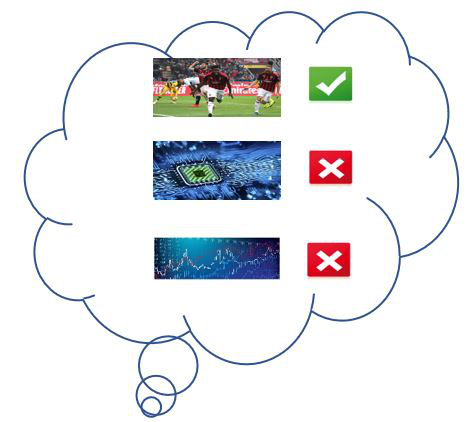
\includegraphics[width=1.8\linewidth]{figures/label.png}
\\

\includegraphics[width=\linewidth]{figures/user.png}
\end{minipage}
\begin{minipage}{0.3\linewidth}
\centering
\vspace{4.5cm}

\includegraphics[width=0.5\linewidth]{figures/info.png} $x_t$
\\
\vspace{-0.3cm}
$\xrightarrow{\hspace*{\linewidth}}$
\\
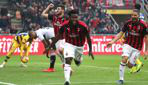
\includegraphics[width=0.5\linewidth]{figures/action.png} $\widehat{y}_t$
\\
\vspace{-0.3cm}
$\xleftarrow{\hspace*{\linewidth}}$
\\

\includegraphics[width=0.3\linewidth]{figures/feedback.png} $z_t$
\\
\vspace{-0.3cm}
$\xrightarrow{\hspace*{\linewidth}}$
\end{minipage}
\begin{minipage}{0.3\linewidth}
\vspace{6cm}
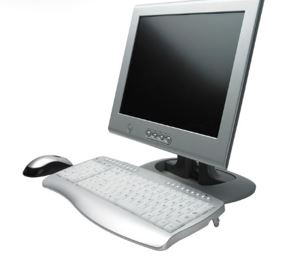
\includegraphics[width=1.2\linewidth]{figures/learner.png}
\end{minipage}
\end{minipage}

\vspace{1cm}
Goal: minimize the total number of mistakes
$\sum_{t=1}^T z_t$.

\vspace*{0.5cm}
Technical assumption: $\| x_t \| \leq 1$ for all $t$.

\section*{Notions of Linear Separability}
Multiclass linear classification: classifier $W = (w_1, w_2, \dots, w_K) \in \R^{K \times d}$ predicts on $x$ by:
\begin{enumerate}
  \item Compute $i$-th score $\ip{w_i}{x}$ for each label $i$
  \item Predict $\hat{y} = \argmax_{i} \ip{w_i}{x}$
\end{enumerate}

\begin{minipage}{0.65\linewidth}
Weakly linearly separable: there exists $W^*$ with $\| W^* \|_F \leq 1$, and for all $(x, y)$:
\begin{align*}
\forall y' \neq y, \quad \ip{w^*_{y}}{x} \ge \ip{w^*_{y'}}{x} + \gamma \; ,
\end{align*}
\end{minipage}
\begin{minipage}{0.35\linewidth}
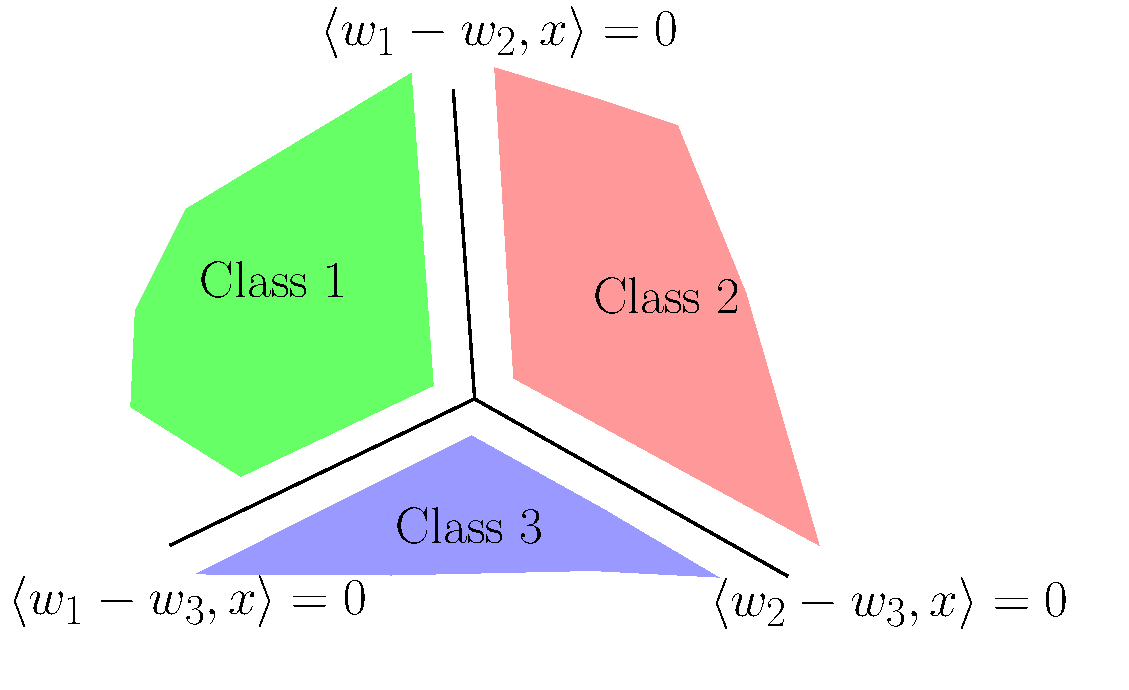
\includegraphics[width=\linewidth]{figures/weak_sep.pdf}
\end{minipage}

\begin{minipage}{0.65\linewidth}
Strongly linearly separable: there exists $W^*$ with $\| W^* \|_F \leq 1$, and for all $(x, y)$:
\begin{align*}
& \ip{w^*_{y}}{x} \ge \gamma/2 \; , \\
\forall y' \neq y, \quad & \ip{w^*_{y'}}{x} \le - \gamma/2 \; .
\end{align*}
\end{minipage}
\begin{minipage}{0.35\linewidth}
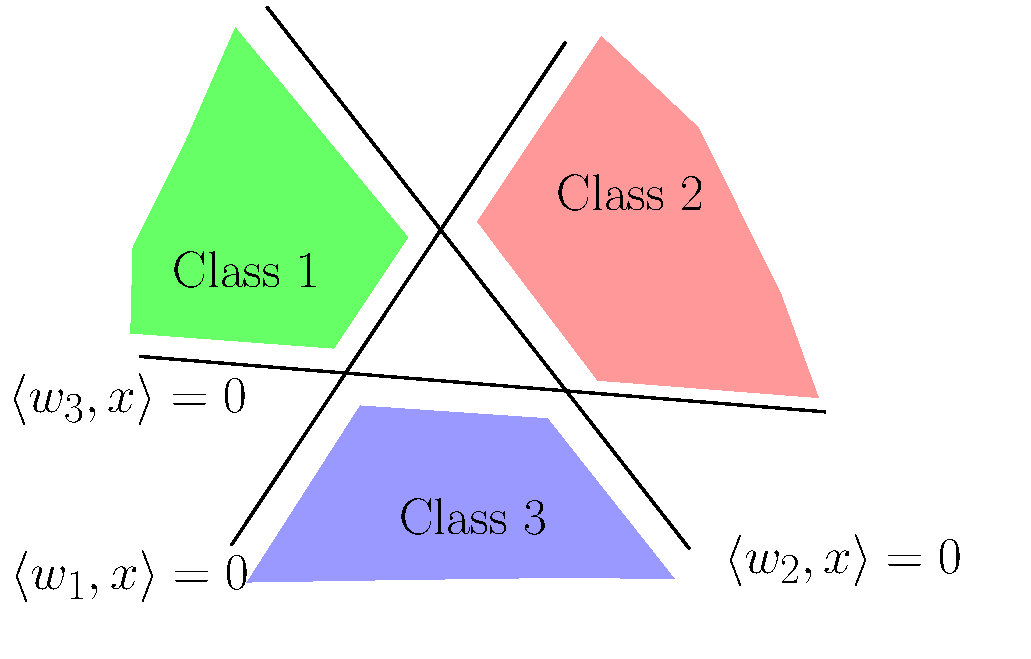
\includegraphics[width=\linewidth]{figures/ova_sep.pdf}
\end{minipage}



%\vspace{-5pt}
\section*{Algorithm}

\textbf{Key idea:}
\begin{enumerate}
\item Create $K$ online classification tasks $T_i, i = 1,\ldots,K$, where task $T_i$ is to predict whether examples belong to class $i$.
%That is, $T_i$ shows examples
%$(x_t, b_t^i)$, where $b_t^i = \begin{cases} +1 & y_t = i \\ -1 & y_t \neq i \end{cases}$.
\item For each task $T_i$, maintain a separate online classification algorithm $\calA_i$.
\item When predicting, aggregate the predictions from all $\calA_i$'s; after receiving the feedback, update all $\calA_i$'s .
\end{enumerate}

\begin{minipage}{0.38\linewidth}
    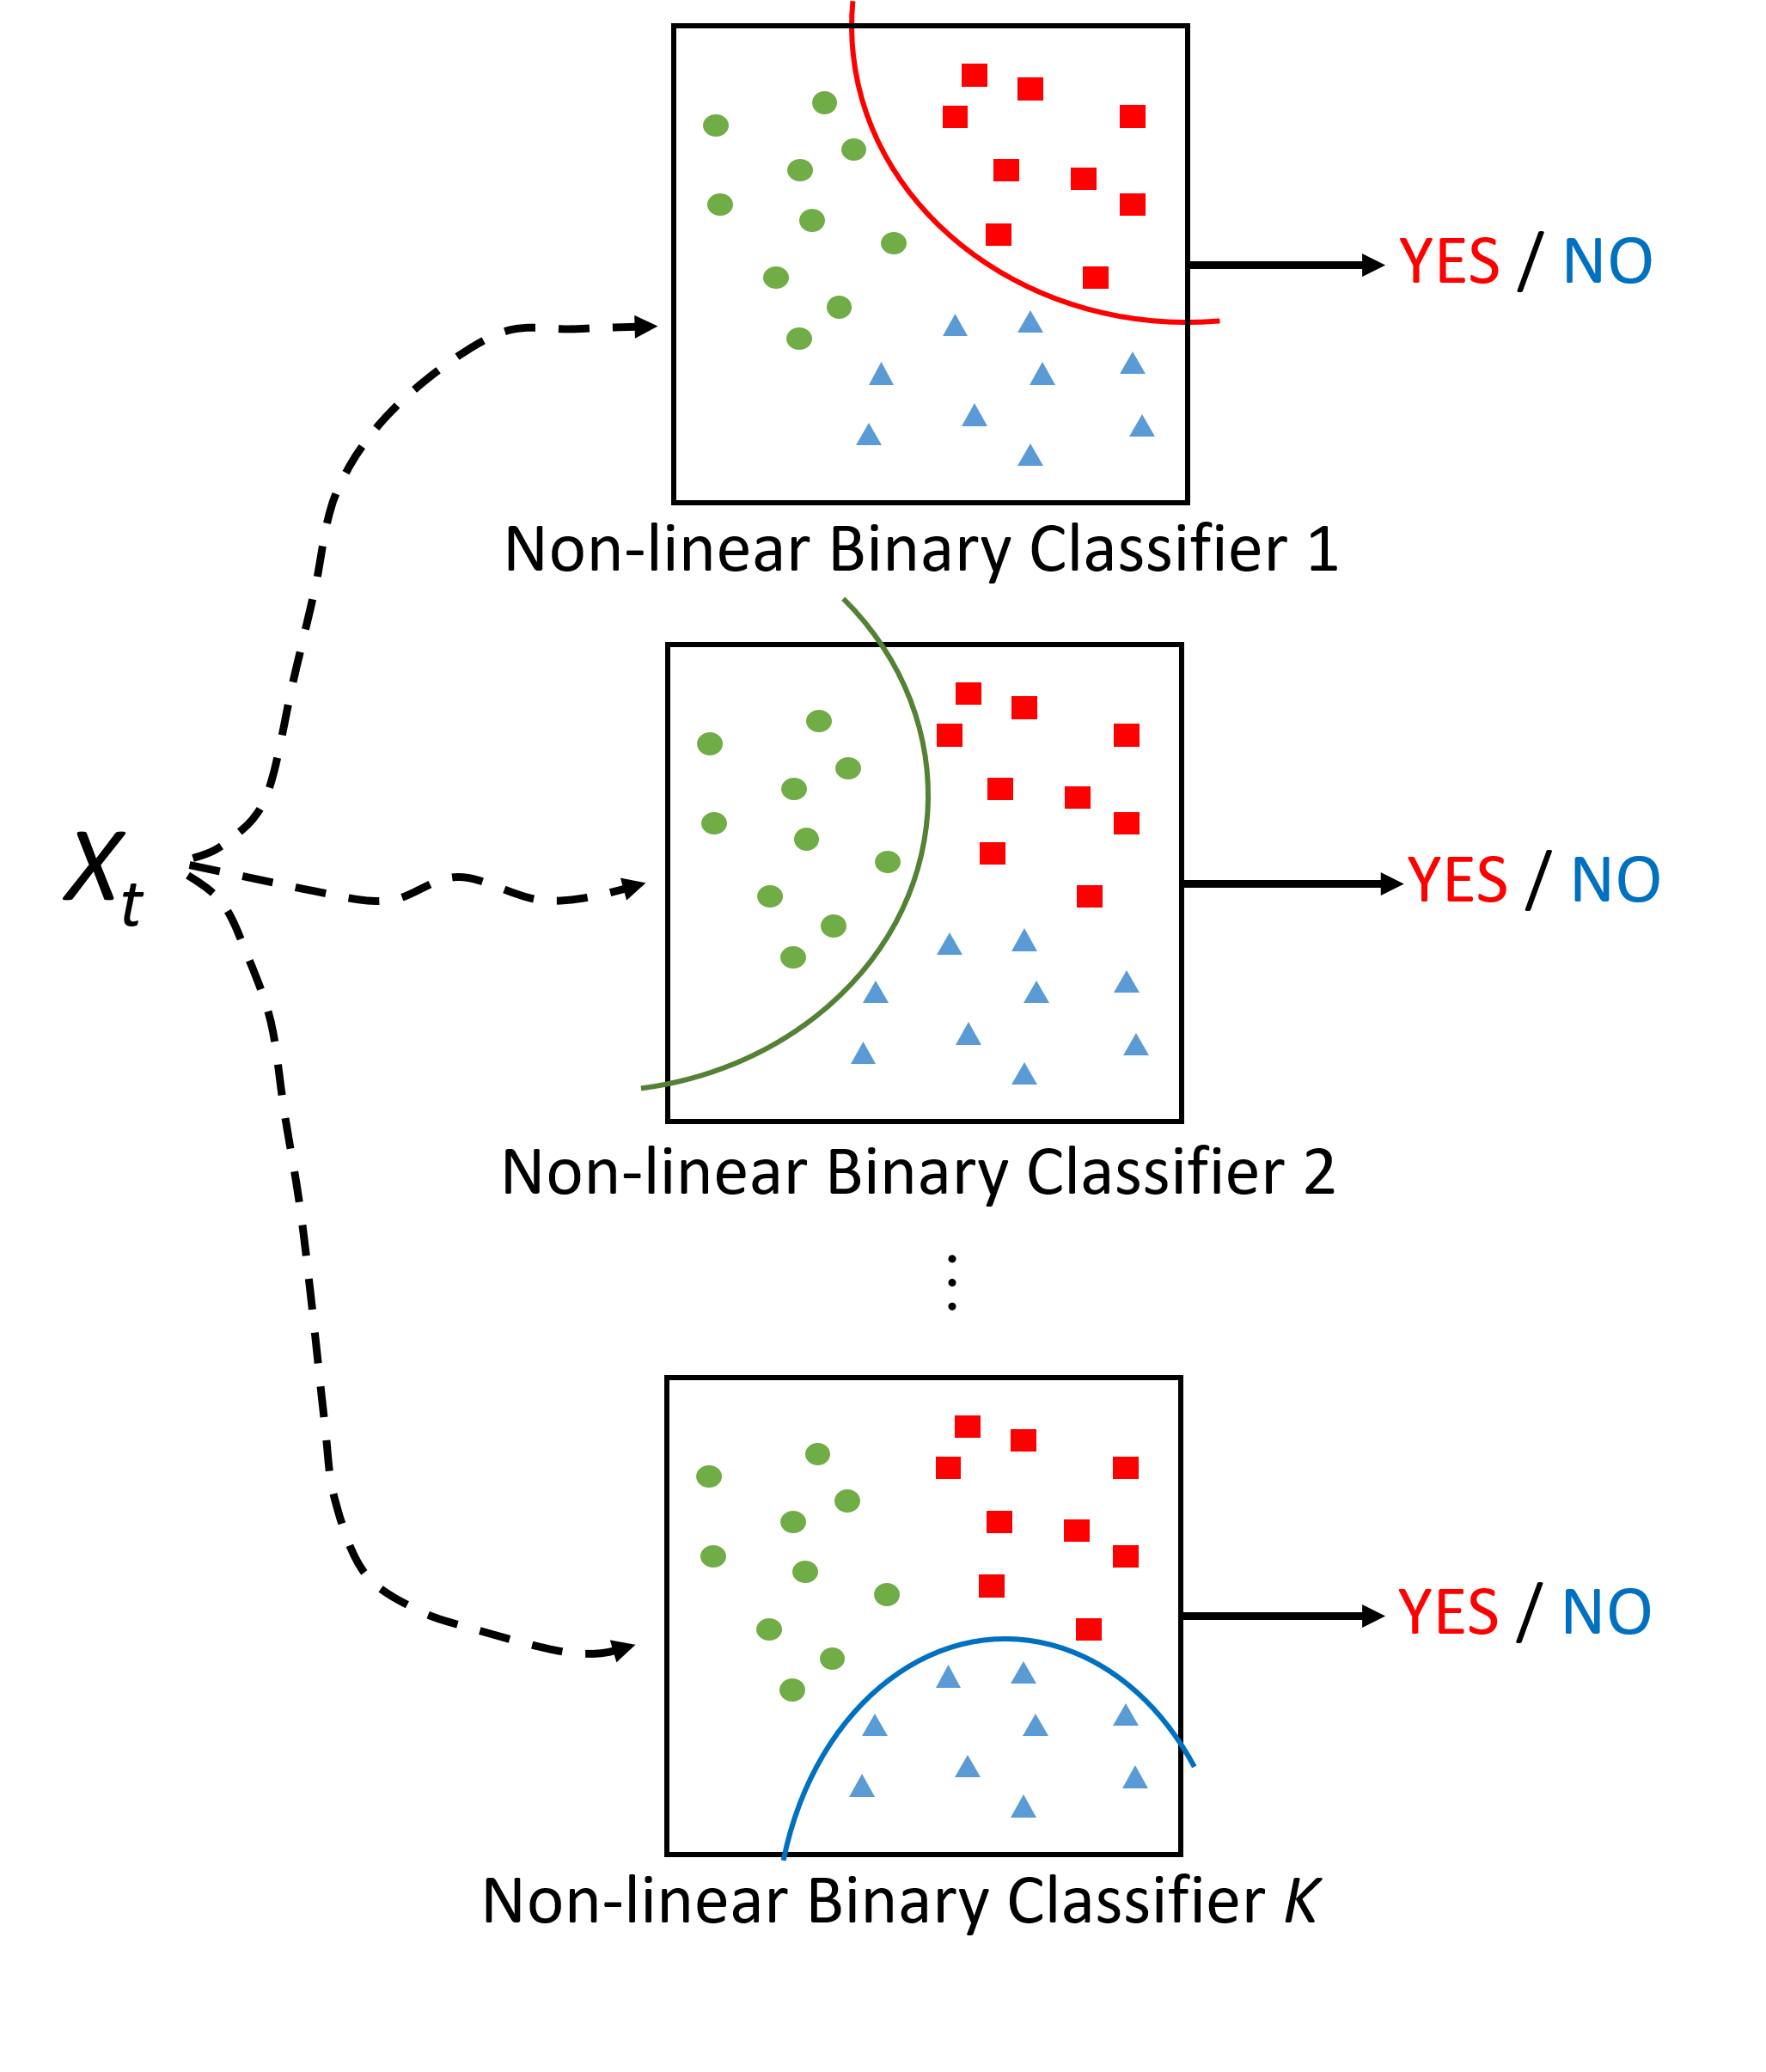
\includegraphics[width=\textwidth]{figures/algorithm.png}
\end{minipage}
\hfill
\begin{minipage}{0.58\linewidth}
    \For{$t=1,2,\dots,T$:}
    {
    Receive example $x_t$.
    \begin{framed}
    \textbf{Query:} For $i = 1,\ldots,K$, ask algorithm $\calA_i$ whether $x_t$ belongs to class $i$.
    \end{framed}
    \begin{framed}
    \textbf{Predict:}\\
    %\begin{enumerate}
    {\color{red} Case 1}: If $\geq 1$ of them respond {\color{red} YES}:\\
    $\widehat{y}_t\leftarrow$ any one of those {\color{red}YES} labels\\
    \\
    {\color{blue} Case 2}: If all of them respond {\color{blue} NO}:\\
    $\widehat{y}_t\leftarrow$ uniform from $\{1,\ldots, K\}$
    \end{framed}
    %\end{enumerate}
    Receive feedback $z_t = \indicator{\widehat{y}_t \neq y_t}$.
   \begin{framed}
    \textbf{Update:}\\
    %\begin{enumerate}
    {\color{red} Case 1}: If $z_t = 1$, send example $(x_t, {\color{blue} \text{NO}})$ to $\calA_{\widehat{y}_t}$.\\
    {\color{blue} Case 2}: If $z_t = 0$, send example $(x_t, {\color{red} \text{YES}})$ to $\calA_{\widehat{y}_t}$.
    %\end{enumerate}
  \end{framed}
  }

\end{minipage}

%\begin{algorithm}[H]
%\begin{framed}
%Initialize $\calA_1, \ldots, \calA_K$. \\
%\For{$t=1,2,\dots,T$}{
%    Observe feature vector $x_t$\\
%    Compute $S_t = \left\{ i ~:~ 1 \le i \le K, \ \calA_i(x_t) = +1 \right\}$\\
%    \If{$S_t = \emptyset$}{
%        Predict $\widehat y_t \sim \text{Uniform}(\{1,2,\dots,K\})$\\
%        Observe feedback $z_t = \indicator{\widehat y_t \neq y_t}$\\
%          \If{$z_t = 0$}
%          {
%            Update $\calA_{\widehat y_t}$ with example $(x_t, +1)$. \label{line:pos-update}
%          }
%     }
%     \Else{
%           Predict $\widehat y_t \in S_t$ chosen arbitrarily \\
%           Observe feedback $z_t  = \indicator{\widehat y_t \neq y_t}$ \\
%            \If{$z_t = 1$}{
%                Update $\calA_{\widehat y_t}$ with example $(x_t, -1)$. \label{line:neg-update}
%            }
%      }
%}
%\end{framed}
%\caption{}
%\label{alg:}
%\end{algorithm}
\vspace*{0.5cm}
\begin{theorem}
If for each $i$, $\calA_i$ makes at most $M_i$ mistakes for task $T_i$, then
our proposed algorithm makes at most $K(M_1 + \ldots + M_k)$ in expectation.
\end{theorem}

\vspace*{0.5cm}
\section*{Performance Guarantees}
\centering
\begin{tabular}{|C{4cm}|C{8cm}|C{10.5cm}|C{10.5cm}|}
\hline
Setting & Sublearner $\calA$ & Sublearner mistake bound & Mistake bound \\
\hline
Strongly linearly separable &
\vspace*{\fill}
Perceptron
\vspace*{\fill} &
\vspace*{\fill}
$O(1/\gamma^2)$
\vspace*{\fill} &
\vspace*{\fill}
$O(K/\gamma^2)$ \quad {\color{red}(tight)}
\vspace*{\fill}
\\
\hline
\vspace*{\fill}
Weakly linearly separable
\vspace*{\fill} &
\vspace*{\fill}
kernel Perceptron with rational kernel $k(x,x') = \frac{1}{1 - \frac 1 2 \ip{x}{x'}}$
%~\cite{Shalev-Shwartz-Shamir-Sridharan-2011}
\vspace*{\fill}
&
\vspace*{\fill}
$2^{\widetilde{O}(\min(K \log^2
(1/\gamma), \sqrt{1/\gamma} \log K))}$
\vspace*{\fill}
&
\vspace*{\fill}
$2^{\widetilde{O}(\min(K \log^2
(1/\gamma), \sqrt{1/\gamma} \log K))}$
\vspace*{\fill}
 \\
\hline
\end{tabular}

\vspace*{1.5cm}
\section*{Related Work - Weakly Linearly Separable Setting}
\centering
\begin{tabular}{|L{14cm}||C{14cm}|C{4cm}|}
\hline
Algorithm & Mistake bound (in Big-$O$) & Efficient? \\
\hline
Halving~\citep{Kakade-Shalev-Shwartz-Tewari-2008} & $K^2(\ln T)/\gamma^2$ or $dK^2 \ln(1/\gamma)$ & No \\
\hline
Minimax algorithm~\citep{Daniely-Helbertal-2013} & \vspace*{\fill}$\min(K/\gamma^2, dK\ln (1/\gamma))$\vspace*{\fill} \quad {\color{red} (tight)} & \vspace*{\fill} No \vspace*{\fill} \\
\hline
Banditron~\citep{Kakade-Shalev-Shwartz-Tewari-2008},
Newtron~\citep{Hazan-Kale-2011},
SOBA~\citep{Beygelzimer-Orabona-Zhang-2017},
OBAMA~\citep{Foster-Kale-Luo-Mohri-Sridharan-2018}
& \vspace*{\fill} at least $\sqrt{KT/\gamma^2}$ or $\sqrt{dKT}$ \vspace*{\fill}
& \vspace*{\fill} Yes \vspace*{\fill} \\
\hline
\end{tabular}
%\lipsum[1]

%Strongly linearly separable setting:\\
%No previous work known???

\section*{Empirical Evaluation}
\begin{flushleft}
\textbf{Experiment 1: strongly separable setting.} Our algorithm with linear Perceptron
and rational kernel Perceptron performs well and exhibit finite mistake bound experimentally.
\end{flushleft}
\begin{figure}[H]
\centering
\begin{subfigure}[b]{0.08\textwidth}
\captionsetup{justification=centering}
\begin{center}
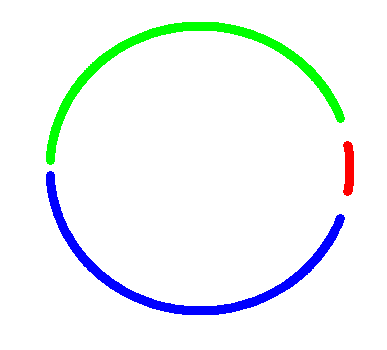
\includegraphics[width=\textwidth, trim={0, 0cm, 0, 0}, clip]{figures/strong_points}
\label{figure:strongly-separable-dataset}
\end{center}
\caption{A strongly separable data distribution with $\gamma = 0.05$.}
\end{subfigure}
\hfill
\begin{subfigure}[b]{0.20\textwidth}
  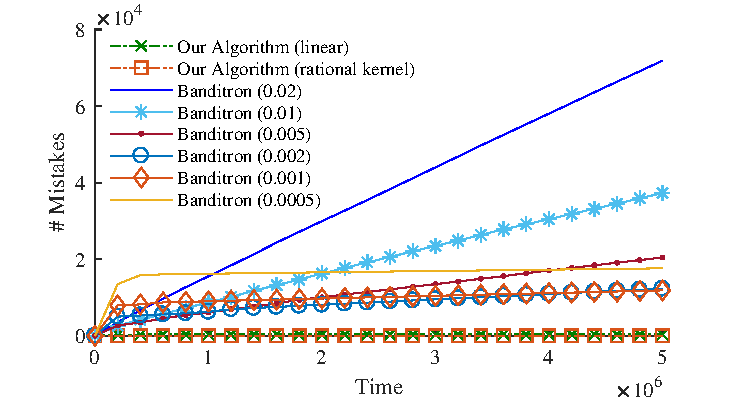
\includegraphics[width=\textwidth]{figures/strong3}
\captionsetup{justification=centering}
\caption{Cumulative number of mistakes as a function of number of examples seen.}
\end{subfigure}
\captionsetup{justification=centering}
%\caption{Left: a strongly separable data distribution with $\gamma = 0.05$. Right: cumulative number of mistakes as a function of iterations.}
\label{figure:strongly-and-weakly-separable-datasets}
\end{figure}
\begin{flushleft}
\textbf{Experiment 2: weakly separable setting.} Our algorithm with rational kernel Perceptron
performs well and exhibit finite mistake bound experimentally.
Our algorithm with linear Perceptron has a high number of mistakes, which is within
expectation.
\end{flushleft}
\begin{figure}[H]
\centering
\begin{subfigure}[b]{0.08\textwidth}
\captionsetup{justification=centering}
\begin{center}

\includegraphics[width=\textwidth, trim={0, 0cm, 0, 0}, clip]{figures/weak_points}
\label{figure:weakly-separable-dataset}
\caption{A weakly separable data distribution with $\gamma = 0.05$.}
\end{center}
\end{subfigure}
\hfill
\begin{subfigure}[b]{0.20\textwidth}
  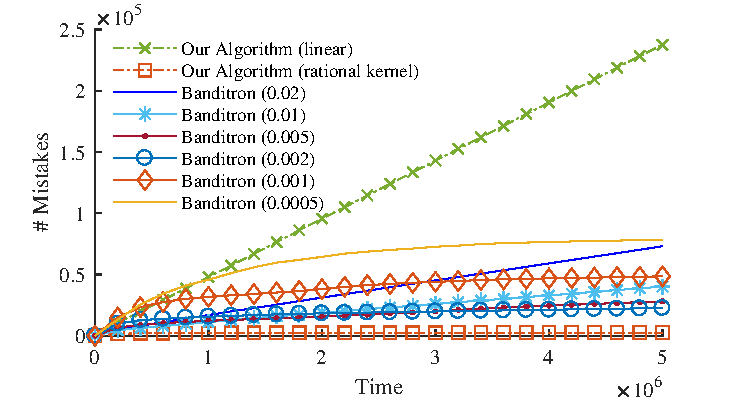
\includegraphics[width=\textwidth]{figures/weak3}
\captionsetup{justification=centering}
\caption{Cumulative number of mistakes as a function of number of examples seen.}
\end{subfigure}
\captionsetup{justification=centering}
%\caption{Left: . Right: .}
\end{figure}

\vspace*{1.5cm}
\section*{Hardness Results}
\begin{enumerate}
      \item Any ``ignorant algorithm'' will make $\Omega(\min\{\sqrt{T}, 2^{\Omega(d)}\})$ mistakes even when the data is strongly linearly separable. An ignorant algorithm does not update itself when it makes a mistake (variants of SOBA~\citep{Beygelzimer-Orabona-Zhang-2017} and OBAMA~\citep{Foster-Kale-Luo-Mohri-Sridharan-2018} are of this type).

    \item Finding a linear classifier that agrees with a labeled dataset and a complementary labeled dataset is NP-hard (naive algorithm requires $2^{\Omega(d)}$ computational complexity).

    A complementary labeled dataset~\citep{ishida2017learning} consists of the following types of examples:
    \begin{align*}
        %(x, y)&: \text{feature $x$ belongs to class $y$}\\
        (x, \overline{y})&: \text{example $x$ does not belong to class $y$}
    \end{align*}

    Observation: finding an intersection of two halfspaces that agrees with a dataset is NP-hard~\citep{Blum-Rivest-1993}.
\end{enumerate}


%----------------------------------------------------------------------------------------
%	REFERENCES
%----------------------------------------------------------------------------------------

	%Use whichever format is typically used by your field. The IEEE and NLM styles are fairly standard.
%If you have any issues with anything feel free to contact the EGS 2016 committee.




%\nocite{*} % Print all references regardless of whether they were cited in the poster or not
\bibliographystyle{plainnat} % Plain referencing style
\nobibliography{biblio} % Use the example bibliography file sample.bib

%\begin{flushright}
%	\LARGE [SCE 000]
%\end{flushright}

%----------------------------------------------------------------------------------------

\end{multicols}
\end{document}
